% Clase 1 — Búsqueda Informada Avanzada
% Lectura: AIMA Sección 3.6
\section{Búsqueda Informada Avanzada}

\subsection{Búsqueda con Memoria Acotada}

\subsubsection{Iterative Deepening A* (IDA*)}
Versión de A* que usa IDDFS con el valor de corte $f(n) = g(n) + h(n)$.
\begin{itemize}
    \item Espacio: $\bigO{bd}$
    \item Completo y óptimo (con $h$ admisible)
\end{itemize}

\subsubsection{Recursive Best-First Search (RBFS)}
Mantiene el mejor valor alternativo $f$ en cada nivel de recursión.
\begin{itemize}
    \item Espacio: $\bigO{bd}$
    \item Puede reexpandir nodos (regenera sub-árboles olvidados)
\end{itemize}

\subsubsection{SMA* (Simplified Memory-Bounded A*)}
Usa toda la memoria disponible; descarta el nodo con mayor $f$ cuando la memoria está llena.

\begin{figure}[H]
\centering
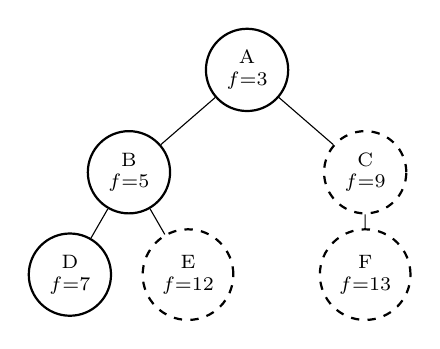
\begin{tikzpicture}[
  nodo/.style={draw=black, thick, circle, minimum size=8mm, font=\scriptsize},
  podado/.style={draw=black, thick, dashed, circle, minimum size=8mm, font=\scriptsize},
  level distance=13mm,
  level 1/.style={sibling distance=30mm},
  level 2/.style={sibling distance=15mm}
]
\node[nodo] {\shortstack{A\\$f{=}3$}}
  child { node[nodo] {\shortstack{B\\$f{=}5$}}
    child { node[nodo] {\shortstack{D\\$f{=}7$}} }
    child { node[podado] {\shortstack{E\\$f{=}12$}} }
  }
  child { node[podado] {\shortstack{C\\$f{=}9$}}
    child { node[podado] {\shortstack{F\\$f{=}13$}} }
  };
\end{tikzpicture}
\caption{IDA* con umbral inicial $f \leq 7$ (el valor de $h$ en la raíz): en la primera iteración se expanden $A$, $B$
y $D$ (todos con $f \leq 7$), y se podan $C$, $E$ y $F$ (nodos punteados, con $f > 7$). Si no se halla la meta, el
umbral sube al menor $f$ podado (aquí $9$) y se repite la búsqueda desde cero.}
\end{figure}

\subsection{Heurísticas: Dominancia y Creación}

\begin{definition}[Dominancia]
$h_2$ domina a $h_1$ si $h_2(n) \geq h_1(n)$ para todo $n$ y ambas son admisibles. Una heurística dominante expande menos nodos.
\end{definition}

Formas de construir heurísticas admisibles:
\begin{enumerate}
    \item \textbf{Relajación del problema}: eliminar restricciones del problema original.
    \item \textbf{Bases de datos de patrones}: precomputar costos exactos de subproblemas.
    \item \textbf{Máximo de heurísticas}: $h(n) = \max(h_1(n), h_2(n))$
\end{enumerate}

\begin{example}[8-puzzle: dos heurísticas admisibles]
    Sea $n$ un estado del 8-puzzle donde las fichas 1, 2 y 3 no están en su casilla objetivo.
    \begin{itemize}
        \item $h_1(n)$ = número de \textbf{fichas fuera de lugar}. Si 3 fichas están mal ubicadas, $h_1(n)=3$.
        \item $h_2(n)$ = suma de \textbf{distancias Manhattan} de cada ficha a su casilla objetivo. Si esas 3 fichas
        están, respectivamente, a 1, 2 y 3 movimientos de su lugar, $h_2(n) = 1+2+3 = 6$.
    \end{itemize}
    Ambas son admisibles (relajaciones del problema: $h_1$ ignora la restricción de que una ficha se mueva solo a una
    casilla adyacente vacía; $h_2$ ignora que solo puede moverse una ficha a la vez). Como $h_2(n) \geq h_1(n)$
    siempre, $h_2$ \textbf{domina} a $h_1$ y expande menos nodos en A*/IDA*.
\end{example}
